\documentclass{scrartcl}
\usepackage{selinput}
\SelectInputMappings{
  adieresis={ä},
  germandbls={ß},
}
\usepackage[ngerman]{babel}

\usepackage{graphicx}
\usepackage[hidelinks]{hyperref}
\usepackage{csquotes}
\MakeOuterQuote{"}
\usepackage{biblatex}

\usepackage{amsmath}
\usepackage{amssymb}

\usepackage{dirtree}
\usepackage{tabularx}

\bibliography{quellen}

\begin{document}

\titlehead{
  Universität Leipzig \\
  Fakultät für Mathematik und Informatik \\
  Institut für Informatik
}
\subject{Projekt Dokumentation}
\title{Generische Methoden für das Faktorisieren und die Berechnung diskreter Logarithmen}
%\subtitle{}
\author{Schindler, Benjamin \and Schmierer, Lukas}
\date{\today}
\publishers{Dr. Claus Diem}
\maketitle

\tableofcontents

\section{Problemstellung}
Diese Projektarbeit, entstanden im Rahmen des Moduls "Mathematische Grundlagen der Kryptographie mit öffentlichen Schlüsseln", beschäftigt sich dem Lösen diskreter Logarithmen und dem Faktorisieren. Wir verwenden dazu sogenannte \emph{generische Methoden}. Diese verwenden ausschließlich allgemeine Gruppeneigenschaften ohne auf die Struktur der zugrundeliegenden Gruppe einzugehen. Es sind zwar asymptotisch schnellere Algorithmen zum lösen des diskreten Logarithmus und zur Faktorisierung bekannt \cite{diem_2011, Adleman_1979}[noch mehr Quellennachweise], jedoch können die hier vorgestellten Algorithmen auf allen endlichen Gruppen [Benny: zusätzlich zyklisch?] angewendet werden. In unserem Projekt arbeiten wir mit Restklassenkörpern, Polynomrestklassenkörpern und darauf aufbauende elliptische Kurven in unterschiedlichen Darstellungen. Die dazu benötigten Grundlagen sind in \cite{Galbraith2012} ausführlich beschrieben. 
\section{Projekt Organisation}
\label{sec:organisation}

\subsection{Verzeichnisstruktur}
\label{sec:verzeichnisstruktur}
Eine Schematische Darstellung der Verzeichnisstruktur ist in Abbildung \ref{fig:verzeichnisstruktur} zu sehen.\\
In unserem Projekt befinden sich drei Verzeichnisse:

\begin{itemize}
\item \emph{tocas} - Enthält den von Dr. Claus Diem bereitgestellten Python Code aus \emph{Tocas} \cite{tocas} unverändert.

\item \emph{ha} - Abkürzung für \emph{Hausaufgaben}. Enthält unsere Python Implementierung zur Lösung der Hausaufgaben aus der Vorlesung "Mathematische Grundlagen der Kryptographie mit öffentlichen Schlüsseln"
\item \emph{projekt} - Enthält den im Rahmen unserer Projektarbeit geschriebenen Python Code zur Lösung des Diskreten Logarithmus Problems und zur Faktorisierung mithilfe generischer Methoden.
\end{itemize}
Da das \emph{tocas}-Projekt separat vorliegt, können dadurch zukünftige Änderungen und Updates in unser Projekt eingepflegt werden. Außerdem erreichen wir so eine strikte Trennung von bereitgestelltem und eigenem Code.\\
Wenn zu bereits existierenden Klassen aus \emph{Tocas} weitere Funktionalitäten hinzugefügt wurden, wurden diese in externe Module geschrieben, die den Datei-Suffix \emph{\_extension} tragen. So verschönert zum Beispiel das Modul \emph{'format\_extension.py'} die Standard-Ausgabe von Tocas (z.B. die Ausgabe für den Ring der ganzen Zahlen mit \( \mathbb{Z} \) statt Z). \\
Innerhalb der Ordner \emph{ha} und \emph{project} befindet sich jeweils ein Unterordner \emph{tests}. In diesem sind verschiedene Tests geschrieben, die mit der Web-Applikation \emph{Jupyter Notebook} aus \cite{jupyterNotebook} ausgeführt werden können.

\begin{figure}[h]
  \fbox{
    \begin{minipage}{0.9\textwidth}
    \dirtree{%
    .1 projekt\_generisches\_faktorisieren\_und\_dlp.
    .2 tocas.
    .3 ....
    .2 ha.
    .3 tests.
    .4 ....
    .3 format\_extension.py.
    .3 ....
    .2 projekt.
    .3 tests.
    .4 ....
    .3 ....
    .2 dokumentation.pdf.
    }
    \end{minipage}
  }
  \caption{Verzeichnisstruktur des Projekts}
  \label{fig:verzeichnisstruktur}
\end{figure}

\subsection{Tests}
\label{sec:tests}

Zu jedem Teilgebiet unseres Projekts wurden zugehörige Tests als Jupyter Notebooks erstellt. Dabei gibt der Name des Tests an, welche Funktionalität getestet wird. Eine Liste aller Tests die wir im Rahmen unserer Projektarbeit geschrieben haben sind inklusive einer kurzen Beschreibung in Tabelle \ref{tab:tests} zu sehen.
\begin{table}[h]
\centering
\begin{tabularx}{\linewidth}{X|p{8.8cm}}
  \begin{minipage}{\linewidth}
      \emph{test\_edwards\_kurven.ipynb} \\
      \emph{test\_weierstrass\_kurven.ipynb}
  \end{minipage} &
  \begin{minipage}{\linewidth}
        \vspace{2pt} Testet grundlegende Funktionalität unserer Realisierung Elliptischer Kurven über endlichen Körpern in den Darstellungen nach Edwards und Weierstrass. \vspace{2pt}
  \end{minipage} \\
  \hline
  \begin{minipage}{\linewidth}
      \emph{test\_pohlig\_hellman.ipynb}
  \end{minipage} &
  \begin{minipage}{\linewidth}
      \vspace{2pt} Testet das Verfahren nach Pohlig und Hellman zur Reduktion endlicher Gruppen in zyklische Untergruppen. 
      Dabei werden auch verschiedene Verfahren zur anschließenden Berechnung  des diskreten Logarithmus ausgeführt.   \vspace{2pt}
  \end{minipage} \\
  \hline
    \begin{minipage}{\linewidth}
    \emph{test\_baby\_step\_giant\_step.ipynb} \\
    \emph{test\_rho.ipynb}  \\
    \emph{test\_kaenguru.ipynb} 
  \end{minipage} &
  \begin{minipage}{\linewidth}
    \vspace{2pt} Testet die von uns implementierten Methoden zu Berechnung des diskreten Logarithmus. Neben dem Baby-Step-Giant-Step-Algorithmus und dem Känguru-Algorithmus (auch Lambda-Methode genannt) 
    werden verschiedene Varianten des Rho-Algorithmus ausgeführt  \vspace{2pt}
  \end{minipage} \\
  \hline
    \begin{minipage}{\linewidth}
    \emph{test\_rho\_faktorisieren.ipynb}
  \end{minipage} &
  \begin{minipage}{\linewidth}
      \vspace{2pt} Testet die Rho-Methode zur Faktorisierung ganzer Zahlen.   \vspace{2pt}
  \end{minipage}
\end{tabularx}
\renewcommand{\arraystretch}{1}
\caption{Übersicht der Jupyter Notebook Tests unserer Projektarbeit}
\label{tab:tests}
\end{table}


\section{Implementierung}
\label{sec:implementierung}

\subsection{Elliptische Kurven}
\label{sec:elliptische_kurven}

Um zu zeigen, dass unsere generischen Methoden auf verschiedenste Gruppen anwendbar sind. Mussten neben den bereits implementieren endlichen Körpern zusätzlich auch rlliptische Kurven über endliche Körper realisiert werden. 
Die in \emph{abstrakte\_gruppen.py} eingeführten Klassen \emph{AdditiveGruppe} und \emph{AdditiveGruppenElement} dienen als Basisklassen unserer elliptischen Kurvengruppen.
Anschließend haben wir uns 2 verschiedenen Darstellungen Elliptischer Kurven bedient, der Edwards-Darstellung und der kurzen Weierstraß-Darstellung. Diese werden in den nachfolgenden Kapitel vorgestellt.
\subsubsection{Edwards Darstellung}
\label{sec:edwards_kurven}

\subsubsection{Weierstraß Darstellung}
\label{sec:weierstrass_kurven}

\subsection{Pohlig Hellman Reduktion}
\label{sec:pohlig_hellman}

modular austauschbarer Algorithmus für die Untergruppen
(als Funktionsparameter)

\cite{Pohlig1978}

\subsection{Baby Step Giant Step}
\label{sec:baby_step_giant_step}

\cite{Galbraith2012}

\subsection{Rho Methode}
\label{sec:rho}

modular walk als parameter

\cite{Galbraith2012}

\subsubsection{Walk Funktion}
\label{sec:walk_funktion}
original und additiv

\subsubsection{Floyd Cycle}
\label{sec:floyd_cycle}

% sqrt(πN/8)

\subsubsection{Brent Cycle}
\label{sec:brent_cycle}

\cite{Brent1980}

\subsubsection{Distinguished Points}
\label{sec:distinguished_points}

% sqrt(πr/2)

\cite{VanOorschot1999}

\subsection{Känguru Methode}
\label{sec:kaenguru}

\subsection{Vergleich zwischen Rho Methoden und Känguru Methode}
Um die theoretischen Annahmen über die Laufzeit der verschiedenen Methoden
zu validieren, wurden Laufzeitmessungen durchgeführt.
Dabei wurde der diskrete Logarithmus \( a = 2778286 \) zu \( g = 3805914789 \)
und \(h = g^a = 2262438373 \) in \( \mathbb{F}_{32416190071} \) gesucht.
Jede Messung 10 mal durchgeführt und die Messwerte anschließend gemittelt.
Die Messergebnisse sind in Tabelle \ref{tab:benchmark} dargestellt und
in Abbildung \ref{fig:benchmark} als Boxplot visualisiert.

\begin{table}[h]
  \centering
  \begin{tabular}{l|c|c|c}
    Methode             & min   & max   & avg   \\ \hline
    Rho (Floyd)         & 1,020 & 2,608 & 1,897  \\ \hline
    Rho (Brent)         & 0,838 & 3,525 & 1,880 \\ \hline
    Rho (Distinguished) & 0,776 & 2,149 & 1,281 \\ \hline
    Känguru             & 1,922 & 1,936 & 1,929
    \end{tabular}
  \caption{Laufzeit verschiedener Rho Methoden und der Känguru Methode in Sekunden}
  \label{tab:benchmark}
\end{table}

\begin{figure}[h]
  \centering
  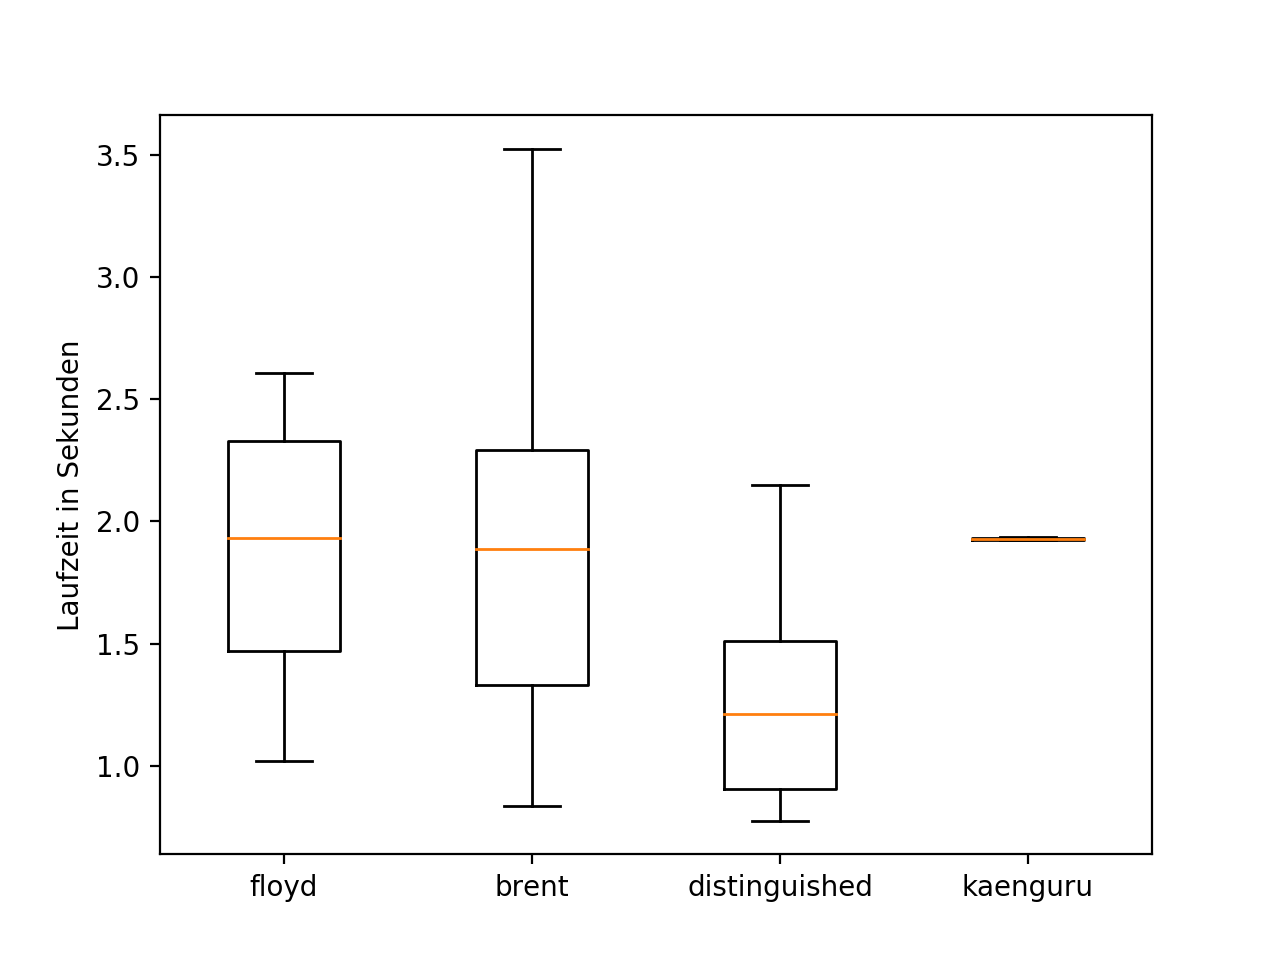
\includegraphics[width=0.8\textwidth]{../projekt/benchmark/plot.png}
  \caption{Grafische Darstellung der Laufzeit verschiedener Rho Methoden und der Känguru Methode}
  \label{fig:benchmark}
\end{figure}

Die Laufzeiten der verschiedenen Methoden verhalten sich gemäß der
theoretischen Annahmen aus Sektionen \ref{sec:floyd_cycle},
\ref{sec:brent_cycle}, \ref{sec:distinguished_points} und
\ref{sec:kaenguru}.
Die \emph{Rho} Methode ist der \emph{Kängeru} Methode überlegen,
wobei die Zyklus Suche mit \emph{Distinguished Points} die durchschnittlich
kürzeste Laufzeit aufweist.

Es lässt sich beobachten, dass die Laufzeitmessungen der \emph{Känguru}
Methode im Vergleich zu den anderen \emph{Rho} Methoden eine geringe Varianz
aufweisen.
Dies lässt sich damit erklären, dass die \emph{walk}-Funktion der
\emph{Känguru} Methode in unserer Implementierung keine zufälligen
Schrittgrößen nutzt und der Algorithmus somit komplett deterministisch
ist.

\subsection{Rho Methode für das Faktorisieren}
\label{sec:rho_faktorisieren}

[schnellere Algorithmen: elliptic-curve factorization method (ECM), Quadratic sieve, General number field sieve]

\cite{Pollard1975}

\newpage
\printbibliography[heading=bibintoc]

\end{document}